%%
%% This is file `sample-manuscript.tex',
%% generated with the docstrip utility.
%%
%% The original source files were:
%%
%% samples.dtx  (with options: `manuscript')
%% 
%% IMPORTANT NOTICE:
%% 
%% For the copyright see the source file.
%% 
%% Any modified versions of this file must be renamed
%% with new filenames distinct from sample-manuscript.tex.
%% 
%% For distribution of the original source see the terms
%% for copying and modification in the file samples.dtx.
%% 
%% This generated file may be distributed as long as the
%% original source files, as listed above, are part of the
%% same distribution. (The sources need not necessarily be
%% in the same archive or directory.)
%%
%% Commands for TeXCount
%TC:macro \cite [option:text,text]
%TC:macro \citep [option:text,text]
%TC:macro \citet [option:text,text]
%TC:envir table 0 1
%TC:envir table* 0 1
%TC:envir tabular [ignore] word
%TC:envir displaymath 0 word
%TC:envir math 0 word
%TC:envir comment 0 0
%%
%%
%% The first command in your LaTeX source must be the \documentclass command.
%\documentclass[manuscript,screen,review]{acmart}
\documentclass[manuscript,review,anonymous]{acmart}
%\documentclass[manuscript,anonymous]{acmart}
%\documentclass[sigconf]{acmart}
\usepackage{subcaption}
\usepackage{balance}  % for useful for balancing the last columns
\usepackage{multirow}
\usepackage{tabulary}
\usepackage{wrapfig}
\usepackage{longtable}
\usepackage{color, colortbl}
\definecolor{Gray}{gray}{0.9}
\usepackage{xcolor}
\usepackage{enumitem}
\usepackage{tablefootnote}
\newcommand{\suggestion}[1]{\textcolor{blue}{#1}}
\newenvironment{itquote}
{\begin{quote}\itshape}
{\end{quote}}

\usepackage{xcolor}
%\usepackage{multirow} % for multirow cells
\usepackage{booktabs} % for better looking tables

%\newcommand{\hl}[1]{\textcolor{blue}{#1}}
\newcommand{\hl}[1]{\textcolor{black}{#1}}
\ifx
\newenvironment{sectionNew}[1]
  {\section[#1]{\textcolor{blue}{#1}}\color{blue}}
  {\normalcolor}
\newenvironment{subsectionNew}[1]
  {\subsection[#1]{\textcolor{black}{#1}}\color{black}}
  {\normalcolor}
\newenvironment{sectionFinished}[1]
 {\section[#1]{\textcolor{blue}{#1}}\color{blue}}
 {\normalcolor}
\fi
\renewcommand{\quote}{\list{}{\rightmargin=\leftmargin\topsep=0pt}\item\relax}
\usepackage{enumitem}
\setlist{nolistsep}
\usepackage[compact]{titlesec}
    \titlespacing{\section}{0pt}{1ex}{0ex}
    \titlespacing{\subsection}{0pt}{0.5ex}{0ex}
    \titlespacing{\subsubsection}{0pt}{0.5ex}{1ex}
    \titlespacing{\paragraph}{0pt}{0.5ex}{1ex}

%%
%% \BibTeX command to typeset BibTeX logo in the docs
\AtBeginDocument{%
  \providecommand\BibTeX{{%
    \normalfont B\kern-0.5em{\scshape i\kern-0.25em b}\kern-0.8em\TeX}}}


\ifx
%% Rights management information.  This information is sent to you
%% when you complete the rights form.  These commands have SAMPLE
%% values in them; it is your responsibility as an author to replace
%% the commands and values with those provided to you when you
%% complete the rights form.
\setcopyright{acmcopyright}
\copyrightyear{2018}
\acmYear{2018}
\acmDOI{XXXXXXX.XXXXXXX}

%% These commands are for a PROCEEDINGS abstract or paper.
\acmConference[Conference acronym 'XX]{Make sure to enter the correct
  conference title from your rights confirmation emai}{June 03--05,
  2018}{Woodstock, NY}
\acmPrice{15.00}
\acmISBN{978-1-4503-XXXX-X/18/06}

\fi
%%
%% Submission ID.
%% Use this when submitting an article to a sponsored event. You'll
%% receive a unique submission ID from the organizers
%% of the event, and this ID should be used as the parameter to this command.
%%\acmSubmissionID{123-A56-BU3}

%%
%% For managing citations, it is recommended to use bibliography
%% files in BibTeX format.
%%
%% You can then either use BibTeX with the ACM-Reference-Format style,
%% or BibLaTeX with the acmnumeric or acmauthoryear sytles, that include
%% support for advanced citation of software artefact from the
%% biblatex-software package, also separately available on CTAN.
%%
%% Look at the sample-*-biblatex.tex files for templates showcasing
%% the biblatex styles.
%%

%%
%% The majority of ACM publications use numbered citations and
%% references.  The command \citestyle{authoryear} switches to the
%% "author year" style.
%%
%% If you are preparing content for an event
%% sponsored by ACM SIGGRAPH, you must use the "author year" style of
%% citations and references.
%% Uncommenting
%% the next command will enable that style.
%%\citestyle{acmauthoryear}

%%
%% end of the preamble, start of the body of the document source.
\begin{document}

%%
%% The "title" command has an optional parameter,
%% allowing the author to define a "short title" to be used in page headers.
%%\title{Exploring the Design and Use of a Card-Based Translational Tool in the Context of Societal Resilience}
%%% alternative titles
%\title{``Where should We Put Our Time and Energy?'': Exploring the Design and Use of a Card-Based Translational Tool to Inform Designs for Societal Resilience}
\title{}

%Understanding the Use of Translational Design Cards in the Context of Societal Resilience

%Exploring the Design and Use of Translational Design Cards in the Context of Societal Resilience

%Exploring the Design and Use of Card-based Translational Tool in the Context of Societal Resilience

%Investigating the Design and Use of Card-based Translational Tool in the Context of Societal Resilience

%Investigating the Design and Use of Translational Design Card in the Context of Societal Resilience

%%
%% The "author" command and its associated commands are used to define
%% the authors and their affiliations.
%% Of note is the shared affiliation of the first two authors, and the
%% "authornote" and "authornotemark" commands
%% used to denote shared contribution to the research.
\ifx
\author{Ben Trovato}
\authornote{Both authors contributed equally to this research.}
\email{trovato@corporation.com}
\orcid{1234-5678-9012}
\author{G.K.M. Tobin}
\authornotemark[1]
\email{webmaster@marysville-ohio.com}
\affiliation{%
  \institution{Institute for Clarity in Documentation}
  \streetaddress{P.O. Box 1212}
  \city{Dublin}
  \state{Ohio}
  \country{USA}
  \postcode{43017-6221}
}

\author{Lars Th{\o}rv{\"a}ld}
\affiliation{%
  \institution{The Th{\o}rv{\"a}ld Group}
  \streetaddress{1 Th{\o}rv{\"a}ld Circle}
  \city{Hekla}
  \country{Iceland}}
\email{larst@affiliation.org}

\author{Valerie B\'eranger}
\affiliation{%
  \institution{Inria Paris-Rocquencourt}
  \city{Rocquencourt}
  \country{France}
}

\author{Aparna Patel}
\affiliation{%
 \institution{Rajiv Gandhi University}
 \streetaddress{Rono-Hills}
 \city{Doimukh}
 \state{Arunachal Pradesh}
 \country{India}}

\author{Huifen Chan}
\affiliation{%
  \institution{Tsinghua University}
  \streetaddress{30 Shuangqing Rd}
  \city{Haidian Qu}
  \state{Beijing Shi}
  \country{China}}

\author{Charles Palmer}
\affiliation{%
  \institution{Palmer Research Laboratories}
  \streetaddress{8600 Datapoint Drive}
  \city{San Antonio}
  \state{Texas}
  \country{USA}
  \postcode{78229}}
\email{cpalmer@prl.com}

\author{John Smith}
\affiliation{%
  \institution{The Th{\o}rv{\"a}ld Group}
  \streetaddress{1 Th{\o}rv{\"a}ld Circle}
  \city{Hekla}
  \country{Iceland}}
\email{jsmith@affiliation.org}

\author{Julius P. Kumquat}
\affiliation{%
  \institution{The Kumquat Consortium}
  \city{New York}
  \country{USA}}
\email{jpkumquat@consortium.net}

%%
%% By default, the full list of authors will be used in the page
%% headers. Often, this list is too long, and will overlap
%% other information printed in the page headers. This command allows
%% the author to define a more concise list
%% of authors' names for this purpose.
\renewcommand{\shortauthors}{Trovato and Tobin, et al.}

\fi
%%
%% The abstract is a short summary of the work to be presented in the
%% article.
\begin{abstract}

\end{abstract}

%%
%% The code below is generated by the tool at http://dl.acm.org/ccs.cfm.
%% Please copy and paste the code instead of the example below.
%%
\begin{comment}

\begin{CCSXML}
<ccs2012>
   <concept>
       <concept_id>10003120.10003121.10011748</concept_id>
       <concept_desc>Human-centered computing~Empirical studies in HCI</concept_desc>
       <concept_significance>500</concept_significance>
       </concept>
 </ccs2012>
\end{CCSXML}

\ccsdesc[500]{Human-centered computing~Empirical studies in HCI}
\end{comment}
%%
%% Keywords. The author(s) should pick words that accurately describe
%% the work being presented. Separate the keywords with commas.
\keywords{}


%%
%% This command processes the author and affiliation and title
%% information and builds the first part of the formatted document.
\maketitle
\section{Introduction}

A missed dose can create a difficult choice: should an older adult manage it independently, or should a family member step in? Family involvement can support medication routines \cite{92}, yet the same checking can shift privacy, responsibility, and control \cite{24,115}. This tension matters especially in many Global South households, where medication work often extends across relatives, shared devices, and intermediated technology use \cite{3,98}. Reminding, purchasing medicines, interpreting prescriptions, and checking doses can therefore be part of everyday family care rather than separate acts of assistance. Medication adherence is more than a problem of remembering. It is also a continuing negotiation over who notices, who acts, and who takes responsibility when a routine breaks down.

Family support can preserve older adults' agency, but it can also redraw its boundaries. Older adults may rely on others for assistance while still wanting control over how support and health information are shared \cite{13,24,30,50}. Interdependence and aging scholarship similarly shows that receiving assistance need not diminish agency because people can rely on others while retaining a meaningful role in how support is arranged \cite{13,30,33}. Yet those boundaries can change across situations: checking may communicate care at one moment and feel like unwanted oversight at another \cite{24,115}. Designing for medication adherence therefore requires support for these shifts without assuming that either independence or family involvement should always take priority.

This negotiation becomes harder when medication technology can act before anyone explicitly asks it to. Mixed-initiative systems have long considered when computational systems should take initiative, while newer proactive agents can intervene in communication or propose actions on a person's behalf \cite{45,52}. In medication care, an AI agent might notice an unconfirmed dose and ask whether a relative should be involved. If the agent keeps the missed dose private, the older adult retains control, but the caregiver may remain unaware. Involving the family can bring support, while also expanding who knows about the dose and who becomes responsible for responding. The AI agent therefore becomes a participant in deciding how responsibility moves between older-adult control and family involvement.

We call this relationship \textbf{allegiance}: whose interests and authority the AI agent gives priority to at a particular moment. Allegiance is not simply a permission setting or a fixed assignment to one user. The same older adult may want private support during an ordinary routine, welcome shared involvement after uncertainty, and resist family intervention in another situation. Because these preferences can shift, allegiance must be visible and revisable rather than hidden in configuration. The design problem is not to align the agent once, but to let people inspect, negotiate, and change whom it serves as circumstances and relationships change.

Care technologies have established that family visibility can support coordination while also redistributing privacy, responsibility, and power. Awareness displays have helped relatives follow older adults' activities and coordinate care \cite{22,82,94}, and collaborative systems have shown how families can participate in person-centred care \cite{81}. Prior studies also show that shared visibility can create new obligations and tensions over who can access information or act on it \cite{24,111,115}. These studies make family participation visible as part of care, not as an external interruption. They leave a further question when the system can itself propose that responsibility move from one person to another.

Research on agent alignment and ways to question automated decisions provides a second foundation for this problem. Alignment research has examined how agents should cooperate with, obey, or represent human objectives \cite{32,38,79}. Work on agents that must account for multiple people's interests further shows how difficult it can be to decide whose interests should take priority \cite{62}. Research on questioning AI decisions, exposing system uncertainty, and revising consent shows how automated actions can remain open to scrutiny and change \cite{6,28,50,71}. Together, these traditions explain why an agent's authority must remain visible and open to revision. What remains unresolved is how that authority is negotiated when an older adult and caregiver both have legitimate, but sometimes different, expectations of what the agent should do.

We study allegiance as an ongoing negotiation rather than a fixed permission or caregiver-access setting. We conducted a two-phase qualitative household study in Bangladesh with 17 older adults and eight family caregivers. Phase 1 examined medication practices and the ways families already shared responsibility. We then developed and deployed a medication-support prototype for two weeks that reminded older adults, recorded medication activity, stated whom it was serving, and requested permission before involving a family member. Post-deployment interviews examined how participants responded to these interactions. Accounts of deployed features were kept separate from judgments about additional mechanisms that were described but not built. Across the study, we analyse when participants treated the agent as a \textbf{tool} for the older adult, a \textbf{coach} shared across the care relationship, or an \textbf{advocate} for greater family involvement. We also examine what made movement among these roles accepted, resisted, or reversed.

Together, these phases trace how responsibility is negotiated before the agent arrives, how allegiance is negotiated after it enters care, and what those negotiations require from design. The study asks:

\textbf{RQ1 (Formative).} How do Bangladeshi older adults and family caregivers distribute and negotiate medication work, and how do they understand responsibility for that work before an agent enters the household?

\textbf{RQ2 (Interaction).} When an agent joins this care network, how do older adults and caregivers negotiate its allegiance, and when are shifts between older-adult control and family involvement accepted, resisted, or reversed?

\textbf{RQ3 (Design).} What makes the agent's roles as tool, coach, or advocate legitimate to older adults and caregivers, and what design implications follow for making shifts among these roles visible, revocable, negotiable, and dignity-preserving?

This work makes three contributions:

\begin{itemize}
  \item \textbf{Empirical.} This study shows how Bangladeshi older adults and family caregivers negotiate medication responsibility and family involvement across formative and post-deployment accounts.
  \item \textbf{Methodological.} We use a caregiver-inclusive household approach that treats caregivers as participants in their own right and preserves divergent accounts of shared medication work.
  \item \textbf{Design.} The study identifies directions for shared-care agents that keep shifts in allegiance visible, negotiable, and reversible.
\end{itemize}

For shared-care agents, whom the system serves cannot remain a hidden configuration choice.

\section{Related Work}

\subsection{Medication Management as Shared Care Work}

Medication adherence is not only about remembering a dose; it is also about coordinating routines, information, and responsibility. Reminder apps can help people notice a dose. Yet studies of older adults and people managing several chronic conditions show that adherence also depends on treatment complexity, daily habits, and how well technology fits existing routines \cite{27,35,107,108}. Medication work can also include interpreting bodily changes, managing health information, and coordinating treatment across people and settings \cite{8,9,54,85,119}. Conversational systems and studies of family health routines extend this view by showing that self-management may involve relatives and care partners rather than one person acting alone \cite{74,92,102,120}. This makes medication management a useful setting for studying how care work is shared.

Shared medication work is easier to understand when care is treated as an ongoing practice rather than a sequence of isolated choices. Practice-oriented HCI describes technology use as part of everyday activity, while care theory emphasizes repeated adjustment to changing needs \cite{61,80,112}. Research on invisible work likewise shows that patients and caregivers spend substantial effort organizing information, monitoring changes, and keeping care moving \cite{8,47,85,106}. Feminist and relational approaches add that care is shaped by responsibility, responsiveness, and relationships, not only by individual choice \cite{10,43,44,72}. Once medication management is viewed this way, the next question is who gets to decide how that work is divided.

Older adults can rely on others without giving up agency. HCI research challenges accounts that treat older adults as passive recipients, reluctant users, or people whose needs can be inferred from age alone \cite{11,41,48,58,59,64,66}. Interdependence research instead shows that people may depend on others while retaining meaningful control over how help is arranged \cite{13,30,78,101}. Studies of technology adoption and home-based care similarly describe agency as shaped through relationships, social position, and information practices \cite{56,86}. The issue is therefore not whether help exists, but whether the older adult still has a meaningful role in shaping it.

Family care makes this tension visible because support and control can move together. Care-network research has long shown that older adults, relatives, and care workers coordinate information and responsibilities across people \cite{22,63,82,94,118}. More recent work on dementia care, home monitoring, and medication support shows that family involvement can improve coordination while also creating disagreements over access, monitoring, and decision-making \cite{24,36,73,76,81,115}. These studies establish that family support can be valuable without assuming that older adults and caregivers always want the same thing.

\textit{What remains unclear is what happens when the system itself proposes a change in this division of work. Prior research explains reminders, family coordination, and relational agency, but gives less attention to how older adults and caregivers respond when an autonomous agent decides that another person may need to become involved.}

\subsection{Family Visibility, Privacy, and Dignity in Later-Life Care}

Family visibility can support care, but it also changes who knows, who acts, and who feels responsible. Awareness displays and connected care tools can help relatives follow an older adult's daily life \cite{22,82,94,118}. Yet monitoring and information-sharing studies show that the same visibility can create conflict over privacy, data ownership, and expectations to intervene \cite{23,24,65,87,111,115}. Research on shared-device privacy reaches a similar conclusion: access rules are often negotiated between people rather than set once by one user \cite{50,122}. This shifts the problem from whether information should be shared to how that sharing changes relationships.

Those relational changes also affect dignity. Older adults may reject technologies that signal decline, and visible assistive devices can affect social standing or the desire to preserve face \cite{17,20,69,73}. Work on domestic robots similarly shows that older adults weigh dignity, autonomy, and the kind of relationship a system appears to create \cite{21}. Goffman's account of self-presentation helps explain why the social meaning of assistance can matter alongside its practical benefit \cite{34}. A system can therefore preserve formal choice and still feel diminishing if it repeatedly presents a person as dependent.

Because these effects are relational, caregiver perspectives matter without replacing the older adult's account. Caregivers often move among several roles and perform work that systems do not fully capture \cite{47}. Studies of home care and security decisions show that caregivers and care recipients can describe the same arrangement differently, including situations where apparently shared decisions leave the older adult with little practical choice \cite{24,56,65,76}. Family information-sharing can likewise improve coordination while creating new privacy concerns for the person receiving care \cite{115}. These differences lead directly to the question of whose interests a system should prioritize when family members disagree.

Autonomy, privacy, dignity, and caregiver coordination each explain part of that problem, but none explains all of it. Autonomy concerns whether the older adult retains meaningful control; privacy concerns what becomes visible and to whom; dignity concerns how support affects social standing; caregiver research explains how responsibilities are distributed. These concepts help identify the stakes. They do not by themselves specify whose interests an autonomous agent should prioritize at a particular moment.

\textit{The gap is therefore not a lack of theories about family care. It is that existing theories do not fully explain how an agent should move between older-adult control and family involvement, or how people judge whether that shift is appropriate in a particular situation.}

\subsection{Family-Mediated Technology Use in Bangladesh}

In Bangladesh, family involvement is not an added layer around care; it is often part of how care is organized. Research on ageing in Bangladesh and South Asia describes limited formal eldercare, strong reliance on relatives, and changing intergenerational arrangements \cite{5,12,37,51,77,90}. An asset-based perspective cautions against describing this only as a lack of formal services, because households and communities already hold practices through which support is provided \cite{60}. This means that an agent entering the household also enters an existing network of family responsibility.

Technology use in that network is often shared as well. Studies in Bangladesh document collaborative phone use, privacy negotiation on shared devices, and privacy risks that arise through ordinary repair and household practices \cite{1,2,3,4}. Research on intermediated technology use shows that one person may operate, explain, translate, or manage a digital resource for another \cite{33,98}. Such support can be a practical way of gaining access rather than evidence that the person receiving help has no agency. Work with rural women in Bangladesh further shows that technology can both reinforce unequal relations and provide ways to exercise agency within them \cite{110}. Shared use therefore makes authority a household issue, not only an interface issue.

Global South HCI explains why these household arrangements should not be measured against an individual-user model by default. Postcolonial computing and critiques of universal design assumptions show how history, infrastructure, and power shape technology use \cite{26,49}. Structural approaches to digital care similarly show that technology can redistribute existing care work rather than simply add a neutral service \cite{53}. Research on sustainable ICTD in Bangladesh, explainable AI in Global South settings, and Global South perspectives on AI governance further shows that systems are interpreted through local institutions, workflows, and stakeholder positions \cite{84,88,96}. Studies of rural clinical AI and voice assistants add that technical adoption does not guarantee a good fit with everyday practice \cite{89,114}. These findings make the household context central to any account of agent authority.

Existing Bangladesh and ICTD work has therefore established shared devices, mediated use, relational privacy, and household power as important design concerns \cite{1,2,3,4,33,98,110}. Across much of this work, however, the technology remains a tool, information system, or shared device rather than an agent that decides when another person should become involved \cite{26,49,53,84,88,96,114}. That difference matters because initiative changes the question. Families must negotiate not only who can use the system, but whose interests should guide what it does.

\textit{What remains underexplored is how older adults and caregivers in such households negotiate authority when an autonomous agent begins acting within existing family care. Our study examines this gap in Bangladesh without assuming that receiving family help means less agency, or that family-based care means everyone will agree.}

\subsection{From Agent Initiative to Allegiance}

An agent becomes part of the care relationship when it can act before anyone explicitly asks it to. Mixed-initiative research established that systems may balance user control with computational initiative, while newer proactive agents can suggest actions, communicate on a user's behalf, or begin support without a direct command \cite{45,52,70}. Research on plan disclosure and AI decision power shows that people care about when an agent acts, how much authority it has, and whether its intended action is visible beforehand \cite{42,55}. Trust research similarly argues that appropriate reliance depends on understanding what a system can and cannot be trusted to do \cite{57,67}. Initiative therefore raises a question of authority, not only capability.

Contestability and oversight research explains how that authority can remain open to challenge. People need ways to question automated actions, intervene, and understand important system boundaries and decision points \cite{6,7,25,28}. Responsibility research further shows that autonomous action can make it harder to determine who should answer for a decision or its consequences \cite{99}. In family care, this problem becomes sharper because involving a caregiver can change privacy and responsibility at the same time. The next question is whose interests should guide that action.

Alignment research provides one answer by asking what an agent should serve. Foundational work distinguishes instructions, preferences, interests, and values, while formal models show that obedience and benefit do not always point in the same direction \cite{32,38,39,79}. More recent pluralistic approaches recognize that agents may face several legitimate values, communities, or principals rather than one user with one stable preference \cite{29,62,105,121}. This work makes the question ``for whom?'' explicit. Much of it, however, remains formal, conceptual, or model-level rather than an account of how related people negotiate an agent's priority during everyday care.

Care technology reaches the same problem from the opposite direction. Multi-stakeholder systems already involve older adults, relatives, professionals, and caregivers, but many focus on awareness, monitoring, information sharing, or coordination \cite{22,24,63,81,82,94,111,115,118}. Conversational systems can also support medication management or communication between older adults and care partners or providers \cite{74,117}. These systems show that several people can have legitimate interests in the same care process. What they offer less evidence about is how a household responds when the agent itself proposes that responsibility move from one person to another.

We use \emph{allegiance} to name that specific interaction problem: whose interests and authority the agent prioritizes at a particular moment. Allegiance is narrower than alignment and different from a permission setting. Autonomy asks whether the older adult retains control; privacy asks what others can see; consent asks whether an action is allowed; alignment asks which instructions, values, or principals guide the agent. Allegiance focuses on how those concerns meet when more than one person has a legitimate claim over what the agent should do. An older adult may want private support in one situation, shared support in another, and no family involvement in a third. The priority can change.

\textit{The central gap is empirical: plural-alignment research identifies the problem of multiple principals, while family-care research documents multiple stakeholders. We still know little about how older adults and caregivers negotiate an agent's changing priority between them during everyday use, or what makes such a shift accepted, resisted, or reversed.}

\subsection{Making Allegiance Visible, Revisable, and Negotiable}

A changing allegiance is only meaningful if people can notice and question the change. Contestable-AI research argues that automated decisions should remain open to human challenge, while work on explanations and oversight shows the value of making plans, limits, and intervention points clear \cite{6,7,25,28,42,52}. For a shared-care agent, this means more than explaining why a reminder appeared. People also need to know when the agent is about to involve someone else and what that involvement will change.

That visibility must be paired with the ability to change one's mind. Research on distributed and interactive consent argues that decisions involving several people require permission that can be discussed, updated, and withdrawn \cite{71,83,104,109,122}. Studies with older adults similarly show that privacy boundaries change with circumstances rather than remaining fixed after setup \cite{50}. Voice interfaces add another difficulty because a short verbal agreement can become routine without remaining meaningful \cite{100}. Rather than treating caregiver access as permanent, shared-care agents therefore need ways for people to reconsider who is involved and under what conditions.

Making role changes visible can also create social costs. Research on stigma, dignity, and self-presentation shows that visible assistance can signal dependence or affect social standing \cite{17,20,21,34,69}. Invisible-work research adds that making care work visible can change the expectations surrounding that work \cite{85,106}. Relational and feminist ethics therefore caution against treating transparency as automatically beneficial \cite{10,43,44}. The design challenge is to make a change clear enough to question without repeatedly presenting the older adult as incapable.

Even small interface cues can shape these relationships. Research on nudging and persuasive design shows that prompts take meaning from the practices in which people receive them \cite{18,31}. Gamification research likewise cautions that points and streaks are not neutral mechanics, while studies of communication and family fitness show that shared metrics can become signals of closeness, obligation, encouragement, or loss \cite{19,40,46,68,91,97}. Self-determination research connects interactive systems to autonomy, competence, relatedness, and motivation, while warning against using these concepts as generic explanations for engagement \cite{14,95,113,116}. The broader lesson is that an agent's signals about responsibility may shape family relationships as well as individual behavior.

These relational shifts also affect how the problem should be studied. Research on reflexive thematic analysis stresses that qualitative interpretation should make analytic choices explicit rather than treating coder agreement as the only sign of quality \cite{15,16,93}. Work on positionality and reflexivity in HCI similarly argues that researchers should account for how their standpoint shapes interpretation \cite{75,103}. This matters when older adults and caregivers may give different accounts of the same care episode. Keeping those accounts distinct allows disagreement to remain evidence rather than being averaged into one household view.

\textit{What remains is a design and methodological gap. We need to understand how an agent's changing allegiance can be made clear, open to withdrawal or reversal, and negotiable without undermining dignity. We also need to study those shifts through the separate accounts of the people affected by them. This is the gap addressed by our caregiver-inclusive household study and by our analysis of the agent as tool, coach, or advocate.}

\section{Method}

\subsection{Study Design}

We conducted a two-phase qualitative household study in Bangladesh from January to June 2026. The study examined how older adults and family caregivers organized medication work within the household and how those arrangements shaped their experiences with a medication-support prototype. All study sessions took place in participants' homes and were conducted in Bangla.

\textbf{Phase 1} consisted of formative interviews, contextual observation, and medication-routine walkthroughs. We examined how medicines were stored and taken, how responsibilities were distributed among household members, how routines were disrupted, and how relatives participated in reminding, checking, purchasing, or otherwise supporting medication use. We conducted a formative analysis of Phase 1 before developing the prototype so that its design reflected practices documented in participating households.

We then developed and installed a medication-support prototype informed by the Phase 1 findings. Participants used the prototype for two weeks. The deployed system provided medication reminders and records, stated whom it was serving, and could ask whether a family member should be involved when a scheduled dose remained unconfirmed.

\textbf{Phase 2} consisted of post-deployment interviews conducted after the two-week deployment. These interviews examined participants' reported experiences with deployed features and their reasoning about several additional design mechanisms that had been specified but were not implemented. We distinguished these forms of evidence throughout the study: accounts of deployed features are treated as reported experiences of use, whereas responses to unimplemented mechanisms are treated as judgments about proposed designs.

We treated the household as the primary context of medication management because relatives often participated in purchasing medicines, reading labels, organizing doses, providing reminders, and checking whether scheduled doses had been taken \cite{106}. Where such coordination occurred, we recruited an involved family caregiver as a participant in their own right. When an older adult and caregiver described the same household event differently, we retained both accounts rather than reconciling them into a single version.

\subsection{Participants and Recruitment}

We recruited participants through snowball sampling, beginning with the research team's social networks and continuing through referrals from friends, colleagues, and community groups. Approximately 30 households were approached. Participation was voluntary and unpaid.

Older adults were eligible if they were at least 65 years old and took medication daily. Family members were eligible if they performed medication-related work for an older adult living in the same household.

The final sample comprised 25 participants: 17 older adults and eight family caregivers. Phase 1 included 16 older adults and eight caregivers, while Phase 2 included 17 older adults and seven caregivers. Sixteen older adults and seven caregivers participated in both phases; one older adult participated only in Phase 2, while one caregiver participated only in Phase 1.

Older adults were 65--80 years old (mean = 69.4; median = 68), including nine women and eight men. Eleven needed large text, including two who could not read, while nine described low or very low smartphone comfort. Five reported taking one medicine daily, three reported eight or more, and one reported thirteen medicines across three dose times.

The eight caregivers included four women and four men. Six reported their age, ranging from 20 to 31 years. Their relationships to the older adults included daughters, sons, a daughter-in-law, and grandchildren. Tables~\ref{tab:older-adults} and~\ref{tab:caregivers} report participant-level demographic, medication, device, and caregiving information.

\begin{table}[t]
  \caption{\textbf{Older adults taking daily medication (n = 17).}}
  \label{tab:older-adults}
  \small
  \begin{tabular}{lrlrrl}
    \toprule
    ID & Age & Gender & Daily medicines & Dose times/day & Deployment device \\
    \midrule
    P01 & 72 & M & 4 or more & 4 & Own smartphone \\
    P02 & 65 & M & 1 & 1 & Household smartphone \\
    P03 & 66 & F & 3 to 4 & 2 & Own smartphone \\
    P04 & 69 & M & 4 & 3 & Own smartphone \\
    P05 & 68 & F & 1 & 1 & Household smartphone \\
    P06 & 67 & M & 1 & 1 to 2 & Household smartphone \\
    P07 & 71 & F & 3 to 4 & 2 or more & Own smartphone \\
    P08 & 67 & F & 2 to 4 & 2 & Household smartphone \\
    P09 & 68 & F & 3 to 4 & 3 & Household smartphone \\
    P10 & 78 & M & 2 & 3 & Own smartphone \\
    P11 & 65 & M & 5 to 6 & 3 & Own smartphone \\
    P12 & 71 & F & 1 & 1 & Own smartphone \\
    P13 & 66 & F & 1 & 1 & Own smartphone \\
    P14 & 66 & F & 5 & Not recorded & Not recorded \\
    P15 & 80 & M & 8 to 10 & 3 & Not recorded \\
    P16 & 76 & F & 13 & 3 & Not recorded \\
    P17 & 65 & M & 8 & 2 & Own smartphone \\
    \bottomrule
  \end{tabular}
\end{table}

\begin{table}[t]
  \caption{\textbf{Family caregivers (n = 8).}}
  \label{tab:caregivers}
  \small
  \begin{tabular}{lrllll}
    \toprule
    ID & Age & Gender & Relation & Older adults supported & Daily medicines managed \\
    \midrule
    C01 & Not recorded & F & Daughter & Mother and father & 3 to 4, and 2 \\
    C02 & Not recorded & F & Daughter & Mother and grandfather & 2 or more, and 3 to 4 \\
    C03 & 21 & M & Son & Father and mother & 3 to 4, and 2 \\
    C04 & 31 & M & Son & Mother & 2 \\
    C05 & 20 & F & Daughter-in-law & Father-in-law and mother-in-law & 4 to 5 \\
    C06 & 22 & F & Granddaughter & Grandmother & 5 to 6 \\
    C07 & 25 & M & Grandson & Grandfather & 10 \\
    C08 & 25 & M & Grandson & Grandmother and mother & 5 to 6 \\
    \bottomrule
  \end{tabular}
\end{table}

\subsection{Phase 1: Formative Household Study}

Following prior situated-practice work \cite{61,9}, Phase 1 examined medication practices before participants encountered the prototype. We used separate semi-structured interview protocols for older adults and family caregivers; the complete protocols are provided in \textbf{Appendix A1} and \textbf{Appendix A2}, respectively.

The interviews covered daily medication routines, medicine storage, disruptions, recent missed or delayed doses, reading and interaction conditions, family involvement, responsibility sharing, technology use, and what happened when the person who usually provided support was unavailable. Rather than asking only about general preferences, we asked participants to reconstruct recent episodes and demonstrate relevant parts of their routines in the places where medication work occurred \cite{61,9}.

The caregiver protocol focused on caregivers' own medication-related work, including how responsibilities developed, how they checked whether medicines had been taken, and what happened when they were unavailable \cite{106}. We distinguished caregivers' accounts of their own activities from their interpretations of the older adult's experience and from jointly described household events.

Each session followed the same general sequence: consent, observation of the immediate setting, semi-structured interviewing, a medication-routine walkthrough, and a closing design reflection. With permission, sessions were audio-recorded in Bangla. Researchers also documented medicine storage, relevant lighting and noise conditions, medication-related artifacts, and household members involved during demonstrations.

Phase 1 supports claims about existing medication practices and the requirements that informed prototype development. It provides no evidence about prototype use.

\subsection{Formative Analysis and Prototype Development}

We conducted a formative analysis of the Phase 1 material before prototype development. The analysis identified requirements concerning timely reminders, medicine and timing information, reduced dependence on manually consulting a schedule, family awareness of unconfirmed doses, simplified interaction, readable presentation, and opportunities for family involvement. After Phase 2, the Phase 1 material was considered again as part of the full qualitative analysis described below.

\begin{figure}[t]
  \centering
  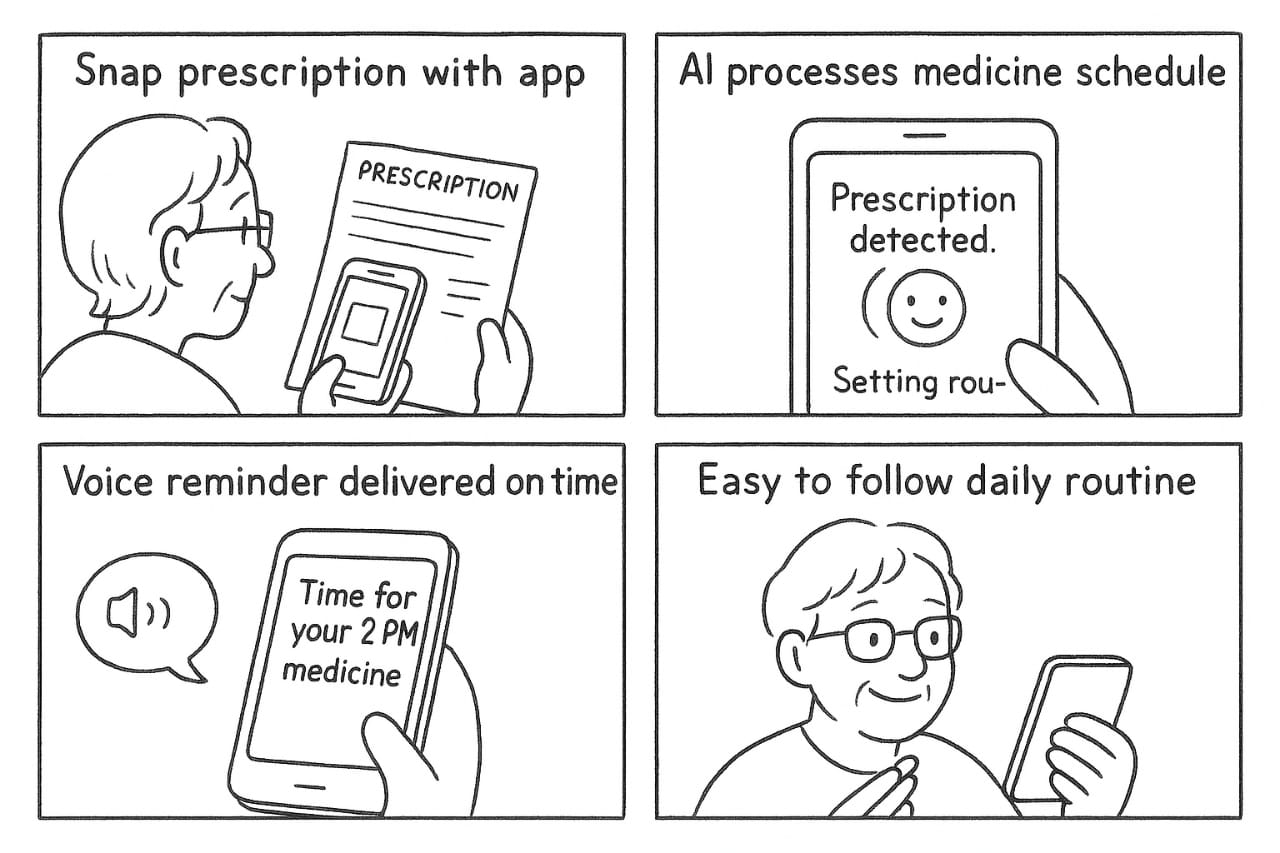
\includegraphics[width=\linewidth]{Figures/initial-uses.jpg}
  \Description{Four-panel storyboard of the design concept: capturing a prescription, the schedule being set from it, a spoken reminder at dose time, and a routine the person can follow.}
  \caption{Four-panel storyboard of the design concept: capturing a prescription, the schedule being set from it, a spoken reminder at dose time, and a routine the person can follow.}
  \label{fig:design-concept}
\end{figure}

Figure~\ref{fig:design-concept} shows how these requirements informed the initial design concept. The concept included prescription capture, schedule creation, spoken reminders, and a medication routine organized around those reminders. Prescription capture was specified in the concept but was not implemented in the deployed prototype.

Participants or family members therefore entered medication schedules manually. At scheduled times, the deployed prototype delivered reminders containing the medicine name and timing. Participants could confirm that a dose had been taken, which updated the medication logbook, streak, and daily heat map.

When a scheduled dose remained unconfirmed, the system could ask whether a family member should be notified. Participants could decline the request, and the family-notification path proceeded only after permission was granted. Medication schedules and changes in whom the system served remained under human control.

The streak and heat map were designed to make medication records visible within the household and create possible occasions for family response. This was a design rationale rather than an assumed effect of the system.

\begin{figure}[t]
  \centering
  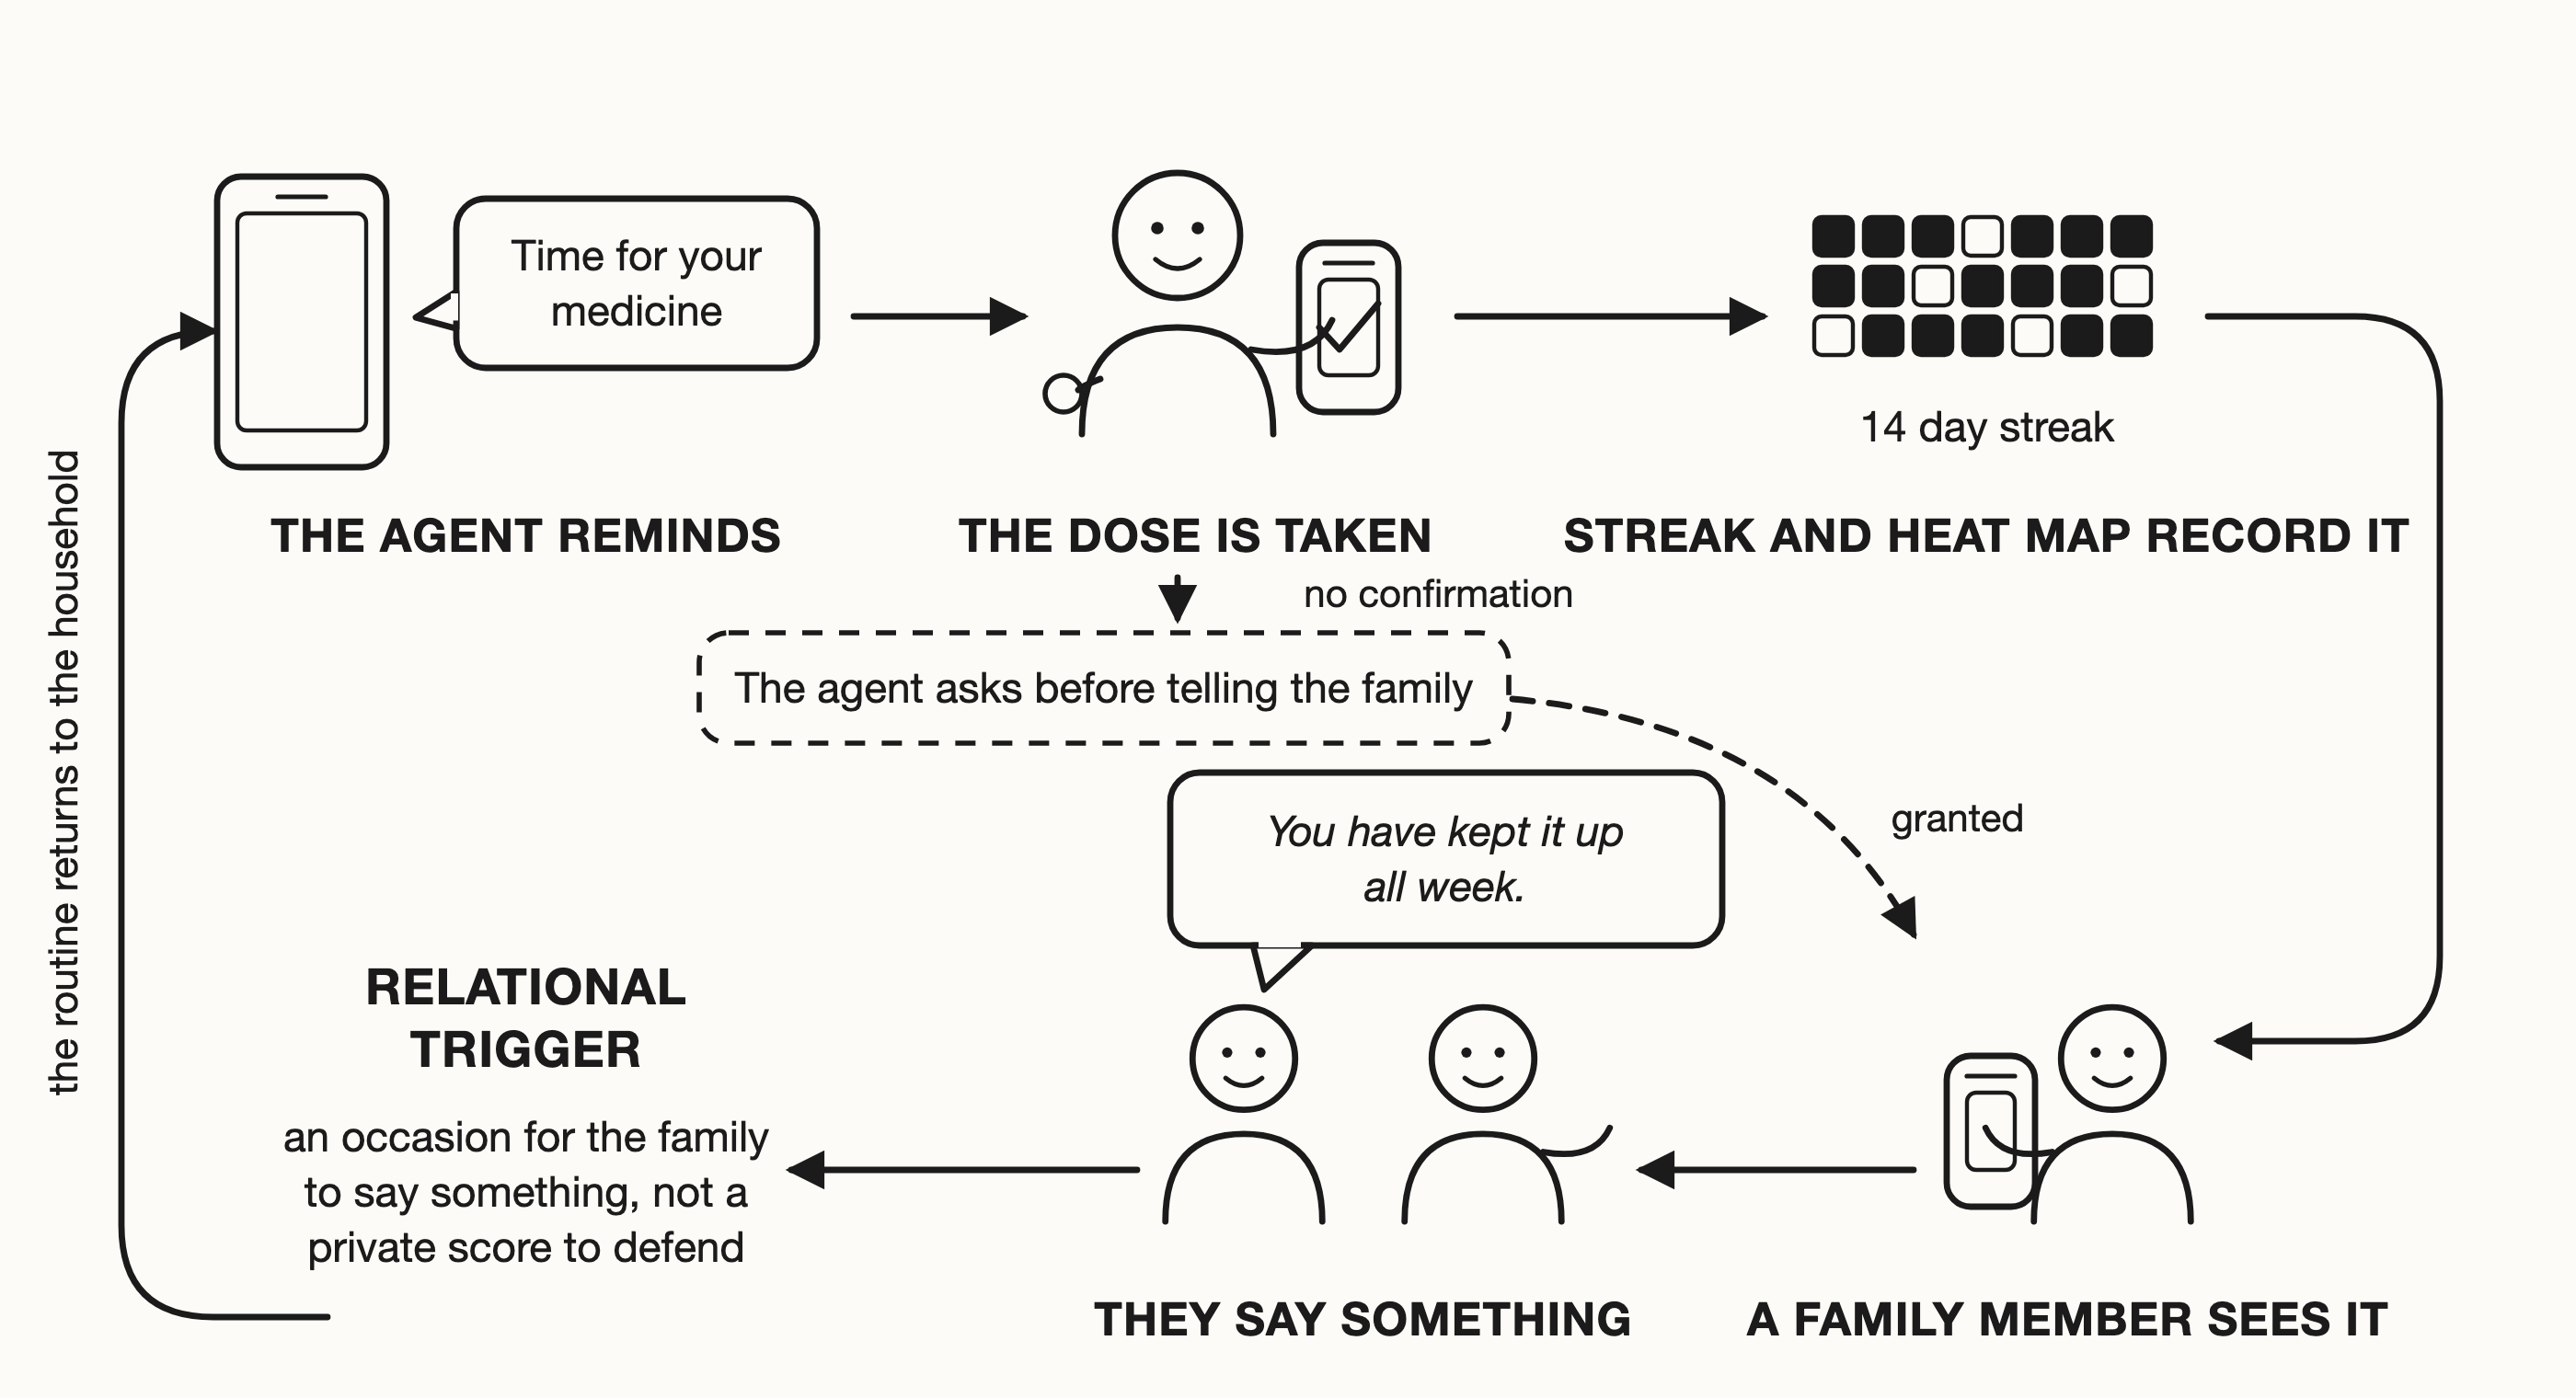
\includegraphics[width=\linewidth]{Figures/relational-trigger-loop.png}
  \Description{Loop diagram: the agent reminds, the dose is taken, a streak and heat map record it, a family member sees the record and says something, and the routine returns to the household. A dashed branch shows an unconfirmed dose reaching the family only after the agent asks and the older adult grants.}
  \caption{Loop diagram: the agent reminds, the dose is taken, a streak and heat map record it, a family member sees the record and says something, and the routine returns to the household. A dashed branch shows an unconfirmed dose reaching the family only after the agent asks and the older adult grants.}
  \label{fig:trigger-loop}
\end{figure}

Figure~\ref{fig:trigger-loop} presents the interaction loop implemented during deployment. After a scheduled reminder, an older adult could confirm taking the dose, which updated the medication record, streak, and heat map. When a dose remained unconfirmed, the family-notification path could proceed only after the participant granted permission.

Four mechanisms in the broader design specification were not implemented in the deployed version: a risk-graded weakening veto, patterned interpretation of silence, a probationary onboarding mode, and shared family scores. These mechanisms were discussed during Phase 2 as proposed designs rather than as features participants had used.

\subsection{Phase 2: Household Deployment and Post-Deployment Study}

\subsubsection{Prototype Deployment}

Researchers installed the prototype during a home visit and configured the initial medication schedule with the older adult or, where relevant, the family member operating the household device. Onboarding covered scheduled reminders, the logbook, and the spoken announcement identifying whom the system was serving.

Nine older adults used personal smartphones, while five used household smartphones shared with or operated by relatives. Device information was unavailable for three participants. We treated shared and intermediated operation as part of the deployment context rather than as equivalent to independent smartphone use, consistent with prior accounts from the region \cite{1,33,98}.

Participants used the prototype for two weeks before the Phase 2 interviews.

\subsubsection{Post-Deployment Interviews}

We returned to participating households after deployment and conducted post-deployment interviews in Bangla. We used separate semi-structured protocols for older adults and family caregivers; the complete protocols are provided in \textbf{Appendix B1} and \textbf{Appendix B2}, respectively. When an older adult and an enrolled caregiver both participated, each discussed the deployment period from their own perspective.

Questions about deployed features covered reminders, announcements of whom the system was serving, medication records, requests for family involvement, occasions when participants accepted or declined those requests, family notifications, and changes participants noticed in their medication routines or family involvement. Interviewers first invited participants to describe experiences in their own terms and then used follow-up probes to reconstruct specific episodes.

The interviews also presented the four mechanisms that were not implemented. These were introduced as hypothetical design possibilities rather than experiences participants were assumed to have had. Several probes described possible interpretations of these mechanisms, so we distinguished episodes or interpretations volunteered by participants from agreement expressed after a probe introduced a possible interpretation. Prompted agreement alone was treated as weaker evidence during analysis.

Accounts of deployed features support claims about participants' reported experiences during the two-week period. Responses to unimplemented mechanisms support only claims about how participants reasoned about the proposed designs.

\subsection{Data Analysis}

\subsubsection{Transcription and Translation}

The verified Bangla transcripts served as the primary analytic record. Automatic speech recognition produced preliminary Bangla transcripts, and machine translation produced initial English renderings, but neither automated output was treated as final. Two Bangla-fluent researchers verified each transcript against the corresponding audio and checked the English rendering against the verified Bangla source. Coding and interpretation were conducted using the Bangla records, and researchers returned to the original Bangla whenever kinship terms, honorifics, relational expressions, or other meanings were not adequately represented in English. Automated systems were used only to support preliminary transcription and translation, not coding, theme development, or interpretation.

\subsubsection{Reflexive Thematic Analysis}

We analysed material from both phases using reflexive thematic analysis \cite{15,16}. Coding began inductively and attended to participants' accounts of medication routines, family involvement, responsibility, technology use, and experiences with the prototype. We worked across semantic and latent levels where relevant and treated themes as researcher-constructed interpretations rather than entities that independently emerged from the data \cite{15,16}.

Analysis began with repeated reading and memoing. The two researchers who conducted the interviews developed preliminary codes and discussed interpretations iteratively with the supervising researcher. We did not calculate inter-rater reliability because coder agreement was not used as a criterion for theme validity within our reflexive approach \cite{16,93}. Researchers then grouped related codes into candidate themes and repeatedly examined them against the underlying transcripts. Themes were revised, combined, separated, or renamed as the analysis developed.

We retained older adults' and caregivers' accounts separately during analysis. When participants described the same household event differently, we treated those differences as part of the data rather than resolving them into a single household account. We maintained analytic memos, coding records, theme maps, and records of cases that complicated developing interpretations. When an interpretation depended on language not adequately represented in English, we returned to the verified Bangla transcript. We make no claim of thematic saturation.

\subsection{Ethical Considerations}

The study received approval from the Brac University Ethics Committee before data collection began. All study procedures followed the approved protocol.

Researchers explained the study purpose, procedures, voluntary nature of participation, audio recording, data use, and automated transcription and translation before obtaining informed consent. Study information was read aloud so participants who could not read received the same information. Consent was obtained individually, and separate permission was requested for audio recording. Caregivers consented independently from the older adults whose medication routines they might discuss.

Personal names were replaced with participant identifiers, and the identifier key was stored separately from the analytic corpus. Participants could discontinue participation at any point.

Three researchers conducted the study. Two conducted the interviews, transcript verification, and coding, while a third supervised the analysis. All three are fluent in Bangla and English. Recruitment began through the research team's social networks, which made some households more reachable than others \cite{75,103}. We therefore do not make population-level claims from the sample.

The two-week deployment supports accounts of participants' experiences during that period rather than longer-term use. We did not measure medication adherence, medication errors, or health outcomes and make no claims that the prototype changed them. Responses to unimplemented mechanisms are similarly limited to participants' judgments about described designs rather than observed use.

% \input{sources/4_findings}
% \input{sources/5_discussion}
% \input{sources/6_conclusion}


\ifx
\begin{acks}
We would like to thank all the participants for their time and for sharing their experiences and perspective with us.
\end{acks}
\fi

\bibliographystyle{ACM-Reference-Format}
\bibliography{reference}

%%
%% If your work has an appendix, this is the place to put it.
\end{document}
\endinput
%%
%% End of file `sample-manuscript.tex'.
